\section{Preliminary definitions}
\subsection{Matrix properties and definitions}
\subsubsection{Trace of a matrix}
\index{Trace of a matrix}
\label{trace}
The \textbf{trace} of a square matrix $\mathbf{A}$, denoted as $\Tr(\mathbf{A})$ is the sum of diagonal elements:
\begin{equation}
\Tr(\mathbf{A}) = \sum_{d=1}^p A_{dd}
\end{equation}
It follows that $Tr(\mathbf{I_d}) = p$.
Also $\Tr(\mathbf{AB}) = \Tr(\mathbf{AB})$ and $\Tr(\x^T\x) = \x^T\x$ the latter being a scalar.

\subsubsection{Exponential matrices}
\label{ExponentialMatrices}
\index{Exponential Matrices}
\begin{definition}{\tb{Exponential matrix}} The matrix exponential is a matrix function on square matrices analogous to the ordinary exponential function. Let $X$ be an $N\times N$ real or complex matrix. Its exponential denoted by $e^X$ is the $N \times N$ matrix given by the power series:
\begin{equation}
e^X = \sum_{k=0}^\infty \frac{1}{k!} X^k
\end{equation}
where $X^0 = I_N$.
\end{definition}

\subsubsection{Similar matrices}
\label{MatrixSimilarity}
\index{Similar matrices}
\begin{definition}{\tb{Similar matrices}}In linear algebra, two $N\times N$ matrices $A$ and $B$ are called \tb{similar} if there exists a $N\times N$ invertible matrix $P$ such that:
\begin{equation}
B = P^{-1}AP
\end{equation}	
\end{definition}
\index{Similar matrices}

\paragraph{\tb{Example}} Similar matrices represent the same linear map under two (possibly) different bases, with $P$ being the change of basis matrix. For example, a rotation around an axis not aligned with the coordinate axis might be difficult to express.  If the axis of rotation is aligned with the positive $z$-axis, then the rotation is simply $S =\begin{bmatrix}\cos \theta &-\sin \theta &0\\\sin \theta &\cos \theta &0\\0&0&1\end{bmatrix}$. So in these new space such a rotation is $y' = Sx'$ where $x'$ and $y'$ are respectively the points before and after the rotation in the new more convenient space. 
In the original space the transformation is $y = Tx$. Then assuming $P$ is the change of base matrix, $T$ can be found as $y' = P y = PTx= S x' \Rightarrow T = P^{-1} S P$.

\subsubsection{Diagonalizable matrices}
\index{Diagonalizable matrices}
\begin{definition}{\tb{Diagonalizable matrices}} In linear algebra, a matrix is called \tb{diagonalizable} if it is similar \autoref{MatrixSimilarity} to a diagonal matrix, i.e., if there exists an invertible matrix $P$ and a diagonal matrix $D$ such that $P^{-1}AP =D$.
\end{definition}

\subsection{Eigenvalue decomposition}
\index{Eigenvalue}
\index{Eigenvector}
\begin{definition}{\tb{Eigenvalues and eigenvector}}
A (non-zero) vector $\vec{v}$ is an \tb{eigenvector} of a square matrix $A \in \CMcal{R}^{N\times N}$ if it satisfies the linear equation:
\begin{equation}
A\vec{v} = \lambda \vec{v}
\label{eigenvector}
\end{equation}
where $\lambda$ is a scalar, termed \tb{eigenvalue} associated to the eigenvector $\vec{v}$. 
\end{definition}
That is, the eigenvectors are the vectors that the linear transformation A merely elongates or shrinks, and the amount that they elongate/shrink by is the eigenvalue.

From this we get an equation for the eigenvalues.
\begin{definition}{\tb{characteristic polynomial} and \tb{characteristic equation}}
\begin{equation}
p(\lambda) = \det\br{A - \lambda I}  = 0
\end{equation}
$p(\lambda)$ is called \tb{characteristic polynomial} and the equation \tb{characteristic equation}.
\end{definition}
$p(\lambda)$ is a $N$-th order polynomial equation in $\lambda$. The set of solution is called \tb{spectrum of $A$}.  
$p(\lambda)$ can be refactored as:
\begin{equation}
p(\lambda) = \br{\lambda - \lambda_1}^{n_1} \br{\lambda - \lambda_2}^{n_2}\cdots \br{\lambda - \lambda_\lambda}^{n_\lambda}
\end{equation}
where $n_i$ is termed the \tb{algebraic multiplicity of the eigenvalue $\lambda_i$}. The number of distinct eigenvalue is $0\le N_\lambda\le N$.

For each eigenvalue we have a specific eigenvalue equation:
\begin{equation}
\br{A-\lambda_i I} \vec{v}= 0
\end{equation}
and there will be $0\le m_i \le n_i$ linearly independent solutions to each eigenvalue equation. The term $m_i$ is termed \tb{geometric multiplicity of $\lambda_i$}, with $m_i \le n_i$, the algebraic multiplicity.

\subsection{Decomposition}
\index{Eigenvalues decomposition}
Eigendecomposition or sometimes spectral decomposition is the factorization of a matrix into a canonical form, whereby the matrix is represented in terms of its eigenvalues and eigenvectors. Only diagonalizable matrices can be factorized in this way. 

Let $A$ be a $N\times N$ square matrix with $N$ linearly independent eigenvectors $q_i$ where $i=1, \cdots, n$. Then $A$ can be factorized as 
\begin{equation}
A = Q \Lambda Q^{-1}
\end{equation}
where $Q$ is  the square $n\times n$ matrix whose $i-th$ column is the eigenvector $q_i$ of $A$, and $\Lambda$ is the diagonal matrix whose diagonal elements are the eigenvalues. The $q_i$ eigenvector are generally normalized but they need not be: the magnitudes of the eigenvectors in $Q$ get cancelled by $Q^{-1}$:
\begin{equation}
A\vec{v} = \lambda \vec{v}\Rightarrow AQ = Q\Lambda \Rightarrow A = Q\Lambda Q^{-1}
\end{equation}
The eigenvalue decomposition gives an easy way to compute power of matrices or exponential matrices:
\begin{equation}
\begin{aligned}
A^{-1} &= Q\Lambda^{-1}Q^{-1}\\
A^n    &=  Q\Lambda^{n}Q^{-1}\\
e^A    &=  Q\left[diag\br{e^\lambda_{ii}}\right]Q^{-1}\\
\end{aligned}
\end{equation}

\subsection{Singular Value Decomposition}
\label{SVD}
It is a factorization of a real or complex matrix that generalizes of the eigendecomposition of a square normal matrix to any $m\times n$ matrix. Given a $m\times n$ real or complex matrix $M$,
\begin{equation}
M = U \Sigma V^*
\end{equation}
where $U$ is a $m \times m$ real or complex unitary matrix, $\Sigma$ is a $m \times n$ rectangular diagonal matrix with non-negative real numbers termed \tb{singular values} on the diagonal and $V$ is a real or complex $n\times n$ unitary matrix. If $M$ is real, $U$ and $V*=V$ are orthonormal matrices, i.e., $U^TU=I$ and $V^TV=I$.

The number of non-zero singular values is equal to the rank of $M$. The column of $U$ and $V$ are called \tb{left singular vectors} and \tb{right singular vectors}. The SVD is not unique. However, it is always possible to choose the decomposition in order to have the singular values in descending order: $\sigma_1 \ge \sigma_2 \ge \sigma_3 \cdots$. In this way $\Sigma$ is uniquely determined, but \tb{not} $U$ and $V$.

In the special case when $M$ is an $m \times m$ real square matrix, the matrices $U$ and $V*$ can be chosen to be real $m \times m$ matrices too. In that case, "unitary" is the same as "orthonormal". Then, interpreting each such matrix $A$ as the linear transformation $x \rightarrow Ax$ of the space $\CMcal{R}^m$, the matrices $U$ and $V*$ represent rotations or reflection of the space, while $\Sigma$ represent the scaling of each coordinate $x_i$ by the factor $\sigma_i$. Thus the SVD decomposition breaks down any invertible linear transformation of $R^m$ into a composition of three geometrical transformations: a rotation or reflection ($V^*$), followed by a coordinate-by-coordinate scaling ($\Sigma$), followed by another rotation or reflection ($U$).

The singular values can be interpreted as the magnitude of the semiaxis of an ellipse in 2D. Singular values encode magnitude of the semiaxis, while singular vectors encode direction. the columns of $U$, $U^*$, $V$, and $V^*$ are orthonormal bases. When the $\mathbf {M}$ is a normal matrix, $U$ and $V^*$ reduce to the unitary used to diagonalize $\mathbf {M}$. However, when 
$\mathbf {M}$  is not normal but still diagonalizable, its eigendecomposition and singular value decomposition are distinct.


\subsubsection{Relationship with eigendecomposition}
\label{SVDEigenDec}
\begin{equation}
\begin{aligned}
M^*M &= V \Sigma^* U^*U \Sigma V^* = V\Sigma^* \Sigma V^*\\
MM^* &= U \Sigma V^*V \Sigma^* U^* = U \Sigma \Sigma^* U^*
\end{aligned}
\end{equation}
The right-hand sides of these relations describe the eigenvalue decompositions of the left-hand sides. The columns of $V$ (right-singular vectors) are eigenvectors of $M^*M$. The columns of $U$ (left-singular vectors) are eigenvectors of $MM^*$. The non-zero elements of $\Sigma$ (non-zero singular values) are the square roots of the non-zero eigenvalues of $M^*M$ or $MM^*$.

Defining the \tb{matrix of principal component variables}
\begin{equation}
Z = U\Sigma
\end{equation}
we can find $Z$ from the eigenvalue-decomposition of $M^*M = W D W^{-1}$.$\Sigma$ is found as explained above. If $W$ is chosen to be orthogonal, then we can set $U=W$, hence we have $Z$.

\subsection{Expectation}
\index{Expectation}
\begin{definition}{\textbf{Expectation}}
Let $X$ be a random variable with a finite number of outcomes $x_1, x_2, \cdots, x_k$ occurring respectively with probabilities $p_1, p_2, \cdots, p_k$. The expectation value is the summation of each outcome times its probability.
\begin{equation}
\E\left[ X\right]= \sum_k x_k \cdot p_k
\end{equation}

In case of an infinite number of outcomes the summation is replaced with the integral:
\begin{equation}
\E\left[ X\right]= \int x \cdot p\left(x \right) dx
\end{equation}
\end{definition}

\href{https://stats.stackexchange.com/a/72614/238980}{As explained here}, when many random variables are involved, and there is no subscript in the $E$ symbol, the expected value is taken with respect to their joint distribution:

$$E[h(X,Y)] = \int_{-\infty}^\infty \int_{-\infty}^\infty h(x,y) f_{XY}(x,y) \, dx \, dy$$


When a subscript is present, in some cases it tells us on which variable we should condition. So

$$E_X[h(X,Y)] = E[h(X,Y)\mid X] = \int_{-\infty}^\infty h(x,y) f_{h(X,Y)\mid X}(h(x,y)\mid x)\,dh  $$

...But in other cases, it tells us which density to use for the "averaging"

$$E_X[h(X,Y)] = \int_{-\infty}^\infty h(x,y) f_{X}(x) \, dx $$


\subsection{Variance}
\index{Variance}
\label{Variance}
\begin{definition}{\textbf{Variance}}
The variance of a random variable $X$ is the expected value of the squared deviation from the mean of $X$:
\begin{equation}
Var\left( X\right) = E\left[ \left( X - \mu \right)^2\right] 
\end{equation}

Variance can be expressed in another way recalling $\mu = E\left[ X\right]$ and using the linearity property:
\begin{equation}
\begin{aligned}
	Var\left( X\right) &= E\left[ \left( X - \mu \right)^2\right] = E\left[ \left( X - E\left[ X\right] \right)^2\right] =\\
	&= E\left[ X^2 - 2\cdot X \cdot E\left[ X\right] + E\left[ X\right] ^2\right]\\
	&= E\left[ X^2\right] - 2\cdot E\left[X \cdot \mu \right]+ E\left[\mu^2\right]\\
	&= E\left[ X^2\right] - 2\cdot \mu \cdot E\left[X\right]+\mu^2 \\
	&= E\left[ X^2\right] - \mu^2 = E\left[ X^2\right] - E\left[ X\right] ^2 \\
\end{aligned}
\end{equation}

\end{definition}

\subsection{Median}
\index{Median}
\begin{definition}{\textbf{Median}}
For any probability distribution on the real line $\R$ with cumulative distribution function $F$, regardless of whether it is any kind of continuous probability distribution, in particular an absolutely continuous distribution (which has a probability density function), or a discrete probability distribution, a median is by definition any real number $m$ that satisfies the inequalities:
\begin{align}
P(x\le m) \ge \frac{1}{2} \quad \text{and} \quad P(x\le m) \ge \frac{1}{2}\\
\end{align}

or equivalently the inequalities
\begin{equation}
\int_{- \infty}^{m} F(x) dx \ge  \frac{1}{2} \quad \text{and} \quad \int_{m}^{\infty} F(x) dx \ge  \frac{1}{2} 
\end{equation}
\end{definition}

\subsection{Median as the minimizer of $L_1$ norm}
%\index{Preliminary definitions!Median as the minimizer of $L_1$ norm}
\label{medianMin}
Assume that $S$ is a finite set, with say $k$ elements. Line them up in order, as $s_1<s_2<\cdots <s_k$.  

If $k$ is even there are (depending on the exact definition of median) many medians. $|x-s_i|$ is the \textit{distance} between $x$ and $s_i$, so we are trying to minimize the sum of the distances. For example, we have $k$ people who live at various points on the $x$-axis. We want to find the point(s) $x$ such that the sum of the travel distances of the $k$ people to $x$ is a minimum.

Imagine that the $s_i$ are points on the $x$-axis. For clarity, take $k=7$. Start from well to the left of all the $s_i$, and take a tiny step, say of length $\epsilon$, to the right. Then you have gotten $\epsilon$ closer to every one of the $s_i$, so the sum of the distances has decreased by $7\epsilon$. 

Keep taking tiny steps to the right, each time getting a decrease of $7\epsilon$. This continues until you hit $s_1$. If you now take a tiny step to the right, then your distance from $s_1$ increases by $\epsilon$, and your distance from each of the remaining $s_i$  decreases by $\epsilon$. So there is a decrease of $6\epsilon$, and an increase of $\epsilon$, for a net decrease of $5\epsilon$ in the sum. 

This continues until you hit $s_2$. Now, when you take a tiny step to the right, your distance from each of $s_1$ and $s_2$ increases by $\epsilon$, and your distance from each of the five others decreases by $\epsilon$, for a net decrease of $3\epsilon$.

This continues until you hit $s_3$. The next tiny step gives an increase of $3\epsilon$, and a decrease of $4\epsilon$, for a net decrease of $\epsilon$.

This continues until you hit $s_4$. The next little step brings a total increase of $4\epsilon$, and a total decrease of $3\epsilon$, for an increase of $\epsilon$. Things get even worse when you travel further to the right. So the minimum sum of distances is reached at $s_4$, the median.

The situation is quite similar if $k$ is even, say $k=6$. As you travel to the right, there is a net decrease at every step, until you hit $s_3$. When you are between $s_3$ and $s_4$, a tiny step of $\epsilon$ increases your distance from each of $s_1$, $s_2$, and $s_3$ by $\epsilon$. But it decreases your distance from each of the three others, for no net gain. Thus any $x$ in the interval from  $s_3$ to $s_4$, including the endpoints, minimizes the sum of the distances. 

In the even case, Some people prefer to say that any point between the two "middle" points is a median. So the conclusion is that the points that minimize the sum are the medians. Other people prefer to define the median in the even case to be the average of the two "middle" points. Then the median does minimize the sum of the distances, but some other points also do.

\textbf{In formulas} consider two $x_i$'s $x_1$ and $x_2$, with $x_2>x_1$
\begin{itemize}
\item \begin{equation}\begin{aligned}
&x_1\leq a\leq x_2
\\ &\sum_{i=1}^{2}|x_i-a|=|x_1-a|+|x_2-a|=a-x_1+x_2-a=x_2-x_1
\end{aligned}\end{equation}
\item \begin{equation}\begin{aligned}
&a < x_1
\\&\sum_{i=1}^{2}|x_i-a|=x_1-a+x_2-a=x_1+x_2-2a\ge x_1+x_2-2x_1\\=&x_2-x_1
\end{aligned}\end{equation}
\item \begin{equation}\begin{aligned}
&a\ge x_2
\\&\sum_{i=1}^{2}|x_i-a|&=-x_1+a-x_2+a=-x_1-x_2+2a\ge -x_1-x_2+2x_2=\\
&=x_2 - x_1
\end{aligned}
\end{equation}

\end{itemize}


$\implies$for any two $x_i$'s the sum of the absolute values of the deviations is minimum when $x_1\leq a\leq x_2$ or $a\in[x_1,x_2]$.

When $n$ is odd,
\begin{equation}
\begin{aligned}
\sum_{i=1}^n\left|x_i-a\right|=\left|x_1-a\right|&+\left|x_2-a\right|+\cdots+\left|x_{\tfrac{n-1}{2}}-a\right| + \left|x_{\tfrac{n+1}{2}}-a\right|+\\
&+ \left|x_{\tfrac{n+3}{2}}-a\right|+ \cdots+\left|x_{n-1}-a\right|+\left|x_n-a\right|
\end{aligned}
\end{equation}
consider the intervals $[x_1,x_n], [x_2,x_{n-1}], [x_3,x_{n-2}], \ldots, \left[x_{\tfrac{n-1}{2}}, x_{\tfrac{n+3}{2}}\right]$. If $a$ is a member of all these intervals. i.e, $\left[x_{\tfrac{n-1}{2}},x_{\tfrac{n+3}{2}}\right],$

using the above theorem, we can say that all the terms in the sum except $\left|x_{\tfrac{n+1}{2}}-a\right|$ are minimized. So
\begin{equation}
\begin{aligned}
\sum_{i=1}^n|x_i-a|&=(x_n-x_1)+(x_{n-1}-x_2)+(x_{n-2}-x_3)+\cdots +\\
& +\left(x_{\tfrac{n+3}{2}}-x_{\tfrac{n-1}{2}}\right) + \left|x_{\tfrac{n+1}{2}}-a\right| = \left|x_{\tfrac{n+1}{2}}-a \right|+\text{costant}
\end{aligned}
\end{equation}

To minimize also the term $\left|x_{\tfrac{n+1}{2}}-a \right|$ it is clear we have to choose $a=x_{\tfrac{n+1}{2}}$ to get $0$ but this is the definition of the median.

$\implies$ When $n$ is odd,the median minimizes the sum of absolute values of the deviations.

When $n$ is even,
\begin{equation}
\begin{aligned}
\sum_{i=1}^n|x_i-a|=|x_1-a|+|x_2-a|+\cdots+\\
+|x_{\tfrac{n}{2}}-a|+|x_{\tfrac{n}{2}+1}-a|+\\
 \cdots+|x_{n-1}-a|+|x_n-a|
\end{aligned}
\end{equation}
If $a$ is a member of all the intervals $[x_1,x_n], [x_2,x_{n-1}], [x_3,x_{n-2}]$, $\ldots$, $\left[x_{\tfrac{n}{2}},x_{\tfrac{n}{2}+1}\right]$, i.e, $a\in\left[x_{\tfrac{n}{2}},x_{\tfrac{n}{2}+1}\right]$,

\begin{equation}
\begin{aligned}
&\sum_{i=1}^n|x_i-a|=(x_n-x_1)+(x_{n-1}-x_2)+(x_{n-2}-x_3)+\cdots + \\
&+\left(x_{\tfrac{n}{2}+1}-x_{\tfrac{n}{2}}\right)
\end{aligned}
\end{equation}

$\implies$ When $n$ is even, any number in the interval $[x_{\tfrac{n}{2}},x_{\tfrac{n}{2}+1}]$, i.e, including the median, minimizes the sum of absolute values of the deviations. For example consider the series:$2, 4, 5, 10$, median, $M=4.5$.

$$
\sum_{i=1}^4|x_i-M|=2.5+0.5+0.5+5.5=9
$$
If you take any other value in the interval $\left[x_{\tfrac{n}{2}},x_{\tfrac{n}{2} + 1} \right] =[4,5]$, say $4.1$
$$
\sum_{i=1}^4|x_i-4.1|=2.1+0.1+0.9+5.9=9
$$

Taking for example $4$ or $5$ yields the same result:
$$
\sum_{i=1}^4|x_i-4|=2+0+1+6=9
$$

$$
\sum_{i=1}^4|x_i-5|=3+1+0+5=9
$$

This is because when summing the distance from $a$ to the two middle points, you end up with the distance between them: $a-x_{\tfrac{n}{2}}+(x_{\tfrac{n}{2}+1}-a) = x_{\tfrac{n}{2}+1}-x_{\tfrac{n}{2}}$

For any value outside the interval $\left[x_{\tfrac{n}{2}},x_{\tfrac{n}{2}+1}\right]=[4,5]$, say $5.2$
$$
\sum_{i=1}^4|x_i-5.2|=3.2+1.2+0.2+4.8=9.4
$$

%%%%%%%%%
\index{Correlation}
\subsection{Correlation}
In statistics, dependence or association is any statistical relationship, whether causal or not, between two random variables or bivariate data. In the broadest sense correlation is any statistical association, though it commonly refers to the degree to which a pair of variables are linearly related.
\begin{definition}{\textbf{Correlation}}
The most familiar measure of dependence between two quantities is the Pearson product-moment correlation coefficient, or "Pearson's correlation coefficient", commonly called simply "the correlation coefficient". It is obtained by dividing the covariance of the two variables by the product of their standard deviations. The population correlation coefficient $\rho_{X,Y}$ between two random variables $X$ and $Y$ with expected values $\mu_X$ and $\mu_Y$ and standard deviations $\sigma _{X}$ and $\sigma_Y$ is defined as
\begin{equation}
\begin{aligned}
\rho_{X,Y}&= \frac{\Cov(X,Y)}{\sigma_X \sigma_Y} = \frac{\E\left[ \br{X -\mu_X} \br{Y -\mu_Y}\right]}{\sigma_X \sigma_Y} = \frac{\E\left[ \br{X -\mu_X} \br{Y -\mu_Y}\right]}{\sigma_X \sigma_Y} =\\
&= \frac{\sum_i^N \br{X_i -\mu_X} \br{Y_i -\mu_Y}}{\sqrt{\sum_i^N(X_i-\mu_X)^2}\sqrt{\sum_i^N(Y_i-\mu_Y)^2}}
\end{aligned}
\end{equation}

An alternative formula purely in terms of moments is
\begin{equation}
\rho_{X,Y} = \frac{  \E\left[ XY \right]     \E\left[ X \right]   \E\left[ Y \right]   }   {\sqrt{\E\left[ X^2\right]-\E\left[ X\right]^2}                      \sqrt{  \E\left[ Y^2\right] -    \E\left[ Y \right]^2} } 
\end{equation}
\end{definition}
The correlation coefficient is symmetric: $corr(X,Y)=corr (Y,X)$. This is verified by the commutative property of multiplication.
It is a corollary of the Cauchy–Schwarz inequality that the absolute value of the Pearson correlation coefficient is not bigger than 1. The correlation coefficient is +1 in the case of a perfect direct (increasing) linear relationship (correlation), $-1$ in the case of a perfect decreasing (inverse) linear relationship (anticorrelation), and some value in the open interval 
$(-1,1)$ in all other cases, indicating the degree of linear dependence between the variables. As it approaches zero there is less of a relationship (closer to uncorrelated). The closer the coefficient is to either $-1$ or $1$, the stronger the correlation between the variables.
If the variables are independent, Pearson's correlation coefficient is $0$, but the converse is not true because the correlation coefficient detects only linear dependencies between two variables.

For example suppose $Y=X^2$. $Y$ is completely determined by $X$ so that they are perfectly dependent but they are uncorrelated.
In the special case where $X$ and $Y$ are jointly normal then "uncorrelatedness" is equivalent to independence.

So correlation might completely miss out non-linear relationships (\autoref{corr}) and furthermore it has nothing to do with the slope.
\begin{figure}
\centering
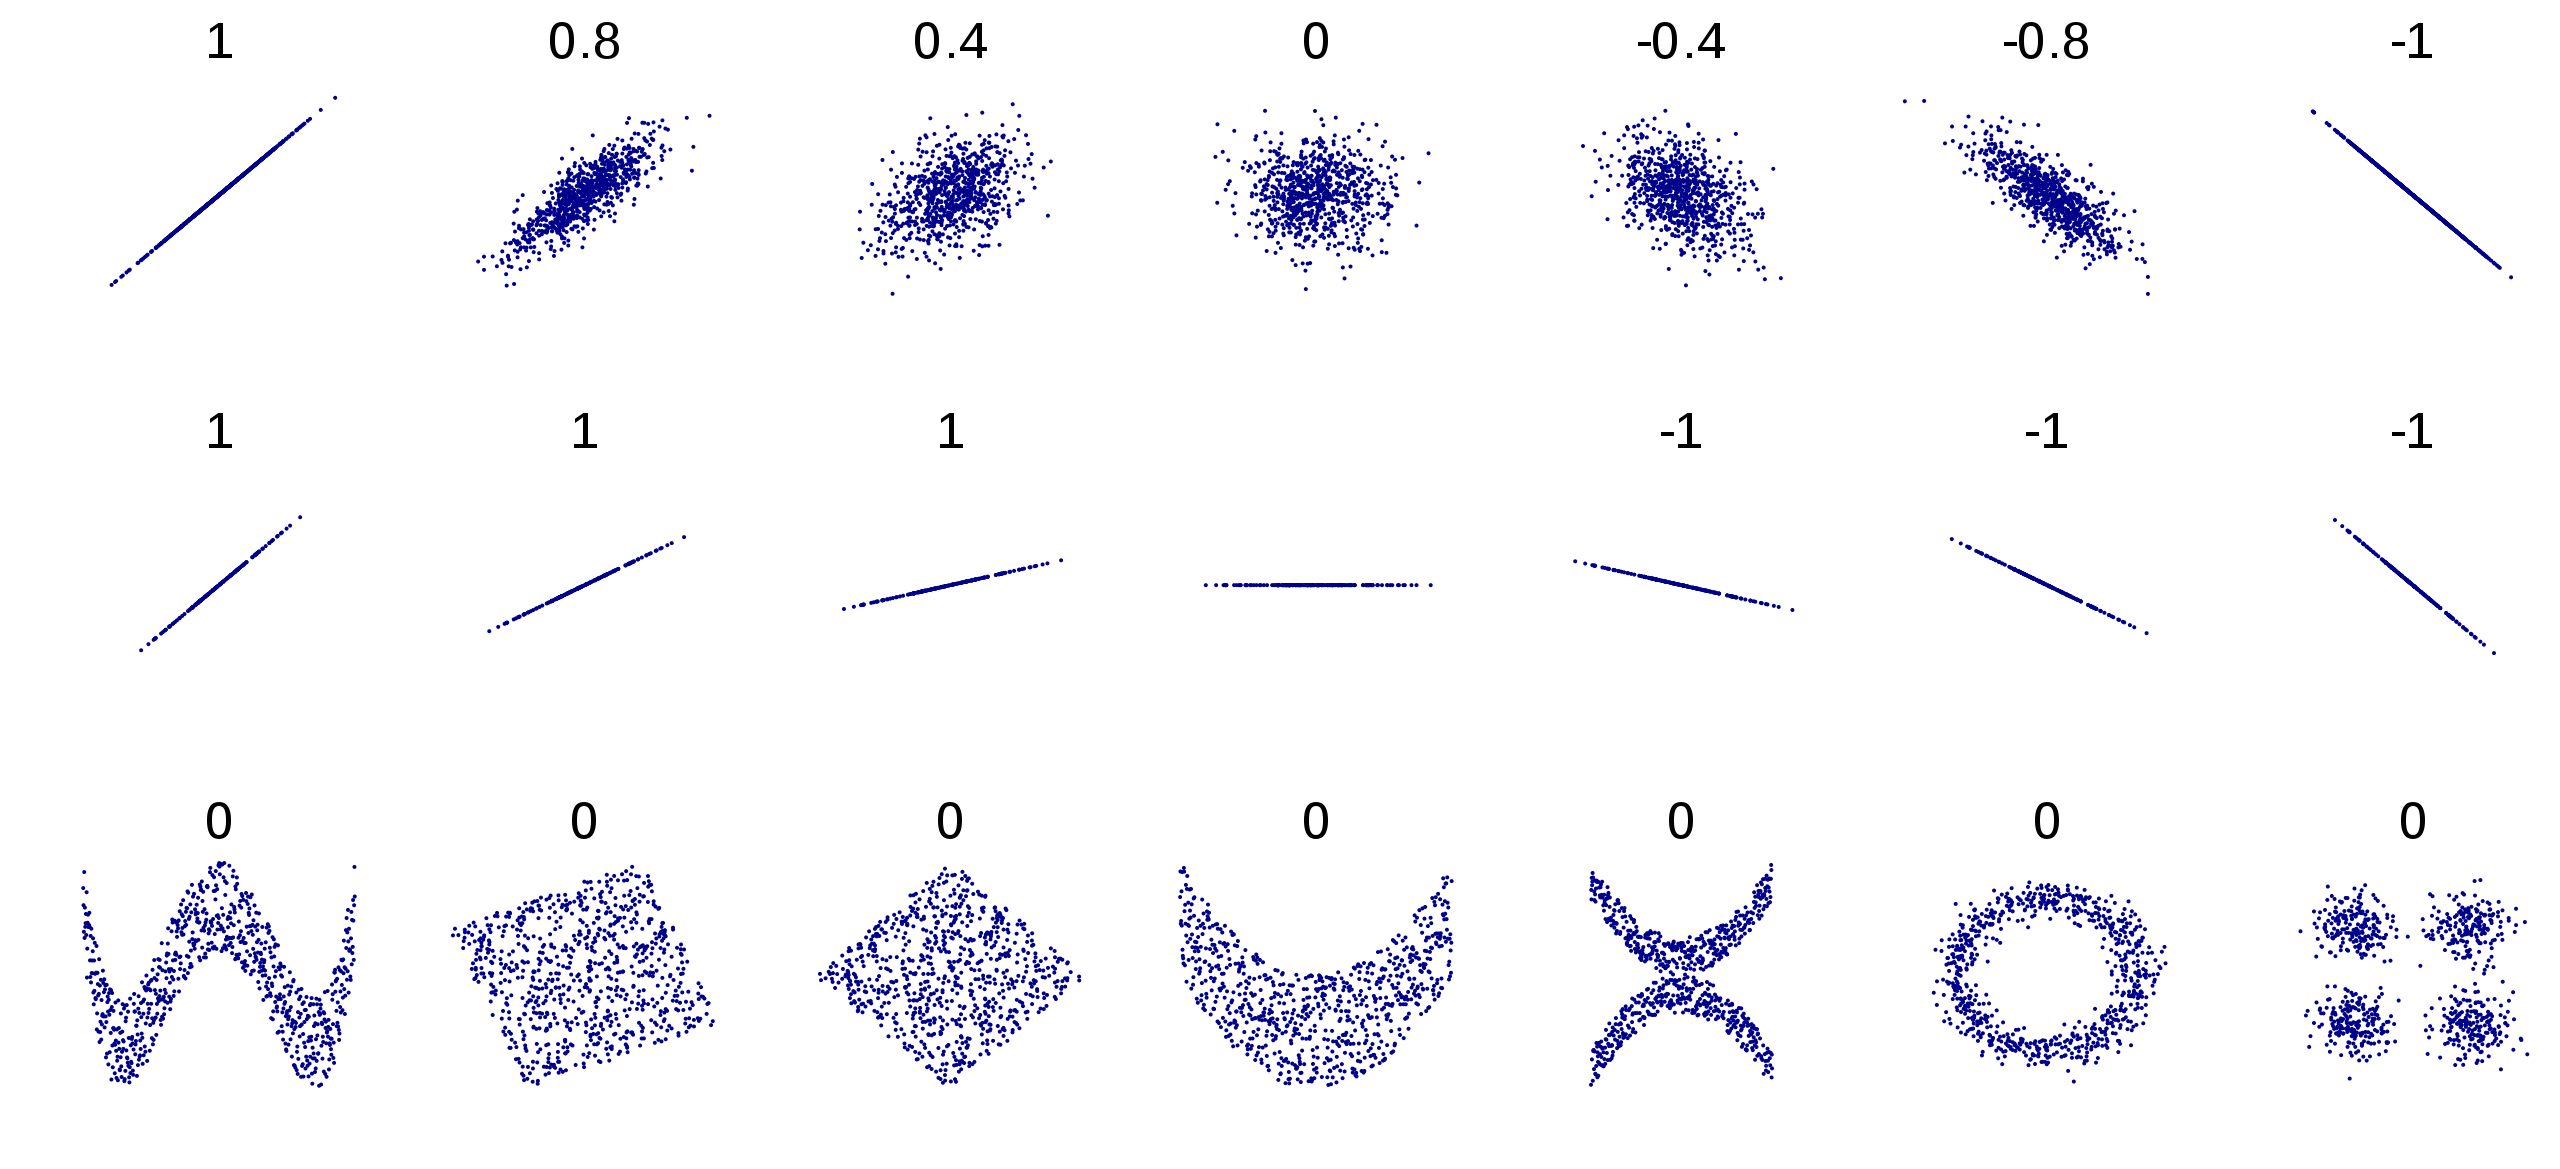
\includegraphics[scale=0.137]{img/corr}
\caption{Plots of correlated and non correlated variables.}
\label{corr}
\end{figure}
\subsection{Gaussian functions and Gaussian distributions}
\index{Gaussian functions}
\index{Gaussian distributions}
\label{gaussian}
\begin{definition}{\textbf{Gaussian function}}
A Gaussian function is a mathematical function in the form:
\begin{equation}
f(x) = a e^{-\frac{(x-b)^2}{2c^2}}
\end{equation}
The Gaussian function has three parameters $a$,$b$ and $c$. The graph of a Gaussian function is the Bell curve. The parameter $a$ is the height of the curve's peak, $b$ is the position of the peak and $c$ the \textit{standard deviation} controls the width of the bell.

An important property of the Gaussian function is that the product of two Gaussian functions is still a Gaussian function:
\begin{equation}
\label{gauss2}
\begin{aligned}
&f(x) \cdot g(x) = a e^{-\frac{(x-b)^2}{2c^2}} a_1 e^{-\frac{(x-b_1)^2}{2c_1^2}} = (a\cdot a_1) e^{-\frac{x^2-2bx+b^2 + x^2-2b_1x+b_1^2}{2c^2 2c_1^2}}=\\
&= (a\cdot a_1) e^{-\frac{2x^2-2x(b+b_1)+ b^2 +b_1^2}{2c^2 2c_1^2}} = (a\cdot a_1) e^{-\frac{x^2-2x\frac{b +b_1}{2}+ \frac{b^2 +b_1^2}{2}}{2c^2 c_1^2}} = \\
&=(a\cdot a_1) e^{-\frac{x^2-2x\frac{b +b_1}{2}+ \frac{b^2 +b_1^2}{2}}{2c^2 c_1^2}} e^{\frac{\br{\frac{b +b_1}{2}}^2 - \br{\frac{b+b_1}{2}}^2 } {2c^2 c_1^2}}=  \\
&=(a\cdot a_1) e^{-\frac{x^2-2x\frac{b +b_1}{2}+\br{\frac{b +b_1}{2}}^2}{2c^2 c_1^2}} e^{\frac{\br{\frac{b +b_1}{2}}^2 - \frac{b^2 +b_1^2}{2}} {2c^2 c_1^2}} = \\
&=(a\cdot a_1) e^{-\frac{\br{x-\frac{b +b_1}{2}}^2}{2c^2 c_1^2}} e^{\frac{\br{\frac{b +b_1}{2}}^2 - \frac{b^2 +b_1^2}{2}} {2c^2 c_1^2}} = \\
&= a_2 e^{-\frac{\br{x-\frac{b +b_1}{2}}^2}{2c^2 c_1^2}} = a_2 e^{-\frac{\br{x-b_2}^2}{2c_2^2}}
\end{aligned}
\end{equation}
\end{definition}

\begin{definition}{\textbf{Gaussian distribution}}
A normalized Guassian function or normal distribution is a Gaussian function with an area under the curve equal to $1$. Hence it can be interpreted as a probability distribution.

To find the formula let us force the curve to have area $1$:

\begin{equation}
\int_{-\infty}^{\infty} a e^{-\frac{(y-b)^2}{2c^2}} dy = a \int_{-\infty}^{\infty} e^{-\frac{(y-b)^2}{2c^2}} dy
\end{equation}
and performing a change of integration variable:
\begin{equation}
\begin{aligned}
&\frac{y-b}{\sqrt{2}c} = x \Rightarrow dx = dy \frac{1}{\sqrt{2}c} dx \Rightarrow dy = \sqrt{2}c dx\\
&a \int_{-\infty}^{\infty} e^{-\frac{(y-b)^2}{2c^2}} dy = \sqrt{2}ac  \int_{-\infty}^{\infty} e^{-x^2} dx 
\end{aligned}
\end{equation}
where  $ \sqrt{2}c$ is a constant so that in can be moved out of the integral. From now on we will focus just on the integral.

Unfortunately the integral has not solutions with elementary functions (Louiville theorem, see Abstract Algebra). However the definite integral exists (demonstration is skipped) and it is:
\begin{equation}
\int_{-\infty}^{\infty} e^{-x^2} dx = \sqrt{\pi}
\end{equation}

To have area equal to $1$ we must have:
\begin{equation}
ac\sqrt{2\pi} = 1 \Rightarrow a =  \frac{1}{\sqrt{2\pi}c}
\end{equation}
So now the function is defined by just 2 parameters. 

Normally $b=\mu$ and is the mean of the function while $c=\sigma$ is the standard deviation.

As opposed to the Gaussian function, multiplying two of these functions we do not get another gaussian distribution, but a scaled guassian distribution. If the Gaussian functions have 0-mean and $\sigma^2=1$ then the product is still Guassian distribution with $0$-mean and $\sigma^2=1$.
\end{definition}

\begin{definition}{\textbf{Standard Normal Gaussian distribution}}
A Standard Normal Gaussian distribution is a Gaussian distribution with $0$ mean and standard deviation $1$.
\end{definition}

\subsection{Hermitian function}
\label{Hermitian}
\begin{definition}{\tb{Hermitian function}}
An hermitian function is a complex function for which its complex conjugate is equal to the original function with the variable changed of sign:
\begin{equation}
\bar{f(x)} = f(-x)
\end{equation}
where the bar indicates the complex conjugate.
From this definition it follows immediately that $f$ is a Hermitian function if and only if:
\begin{itemize}
\item the real part of $f$ is an even function;
\item the imaginary part of $f$ is an odd function.
\end{itemize}
\end{definition}

\subsection{Non-negative definite kernels}
\begin{definition}{\tb{Non-negative definite kernels}}
$K$ is said to be non-negative definite (or positive semidefinite) iff
\begin{equation}
\sum _{i=1}^{n}\sum _{j=1}^{n}K(x_{i},x_{j})c_{i}c_{j}\geq 0
\end{equation}
for all finite sequences of points $\forall x_i,x_j \in \CMcal{X}$ and $\forall c_i, c_j \in \CMcal{R}$.
\end{definition}